\begin{sidewaysfigure*}
\thisfloatpagestyle{mylandscape}%
\rotatesidewayslabel%
\centering
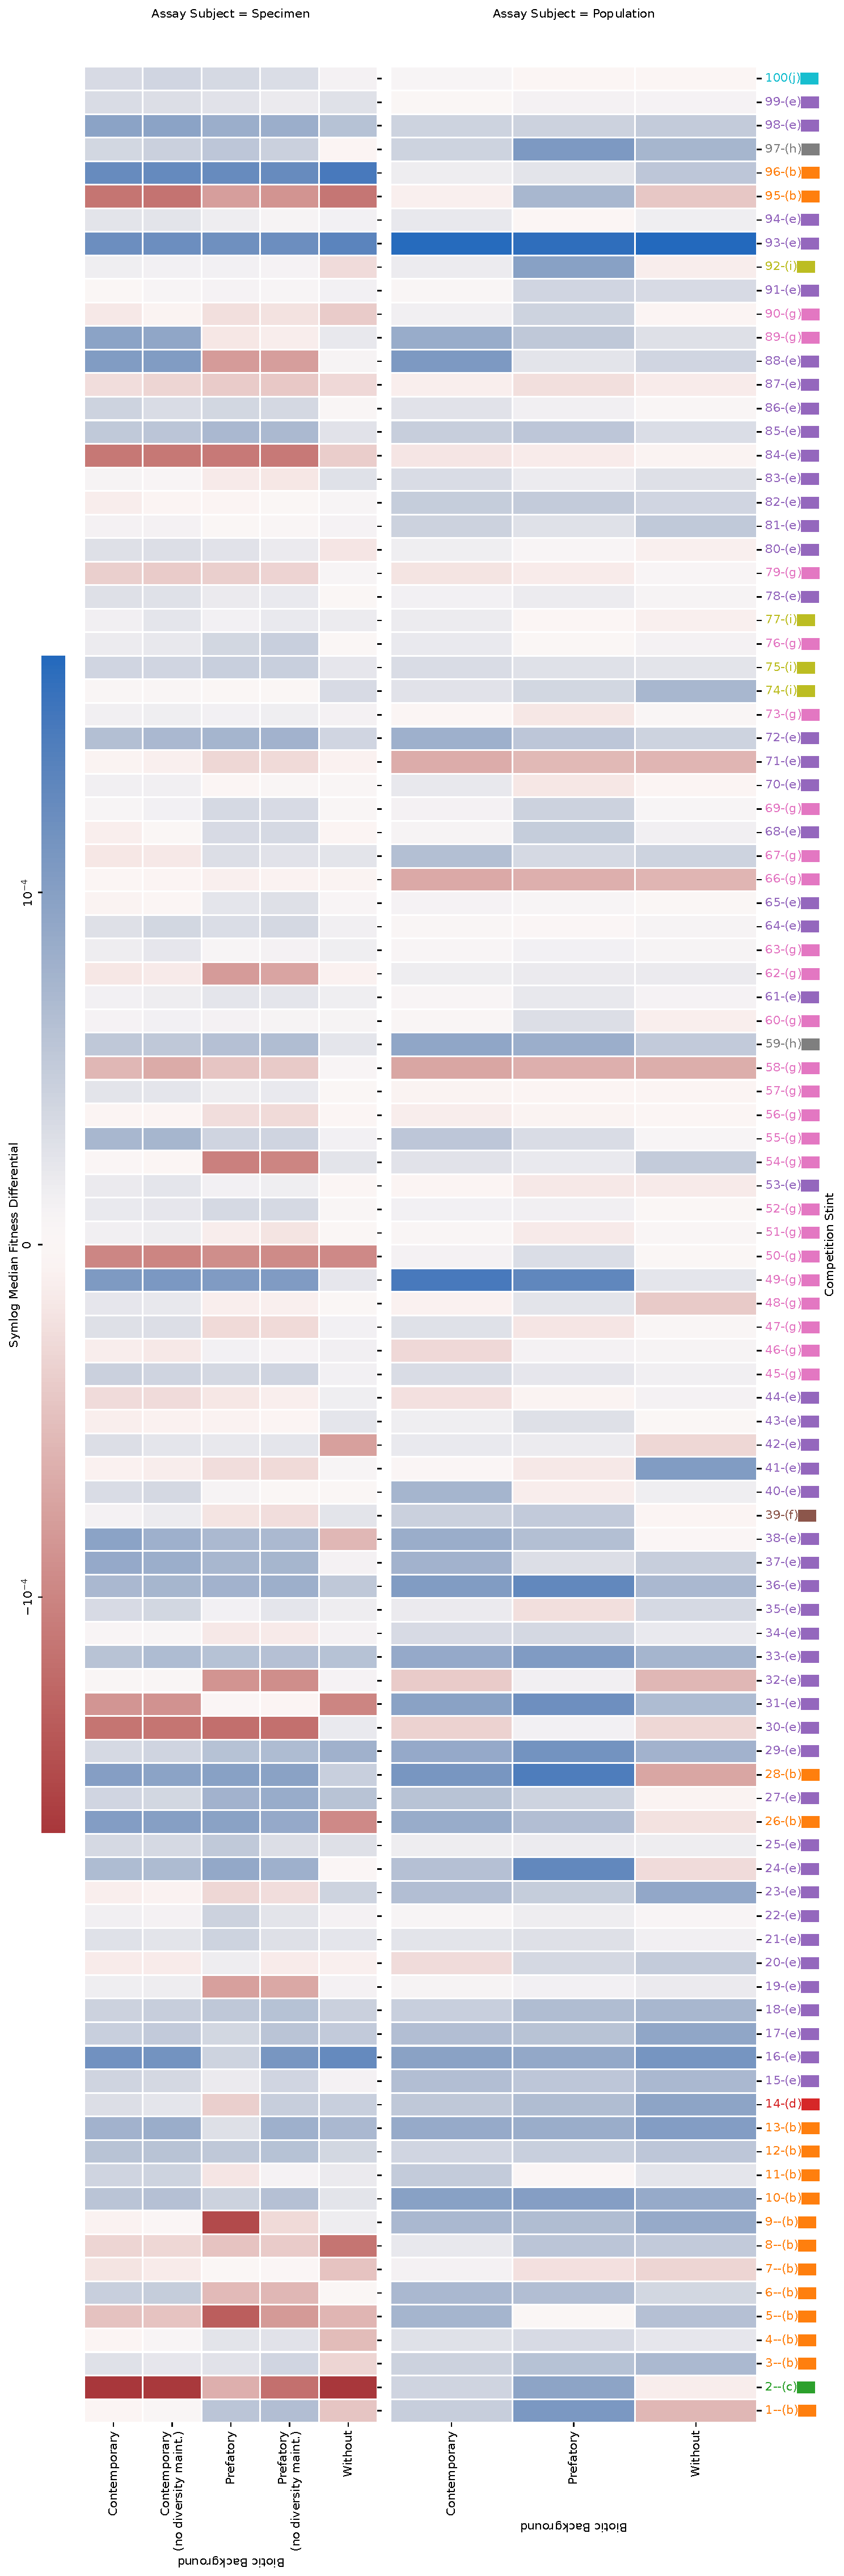
\includegraphics[width=\linewidth]{{submodule/dishtiny/binder/bucket=prq49/a=adaptation_assays+endeavor=16/teeplots/hue=symlog-median-fitness-differential+viz=facet-heatmap+x=biotic-background+y=competition-stint+ext=}}

\caption{
\textbf{Adaptation assay effect strengths.}
\footnotesize
Median calculated fitness differential outcomes of competition experiments.
Zero fitness differential corresponds to a neutral result, color mapped to white.
Blue indicates positive fitness differential (fitness gain) compared to the previous stint and red indicates negative fitness differential (fitness loss).
Color coding and parentheticals of stint labels correspond to qualitative morph codes described in Table \ref{tab:morph_descriptions}.
Note that color intensity is plotted on a symlog scale due to distribution of fitness differentials over multiple orders of magnitude.
Upper panels shows results for sampled focal strain genome, lower panel shows results for entire focal strain population.
See Figure \ref{fig:adaptation_assay_cartoon} for explanation of competition biotic backgrounds.
}
\label{fig:median_fitness_differential_symlog}
\end{sidewaysfigure*}
